\section{Transport Layer}
\paragraph{Schicht 4: Transportschicht}

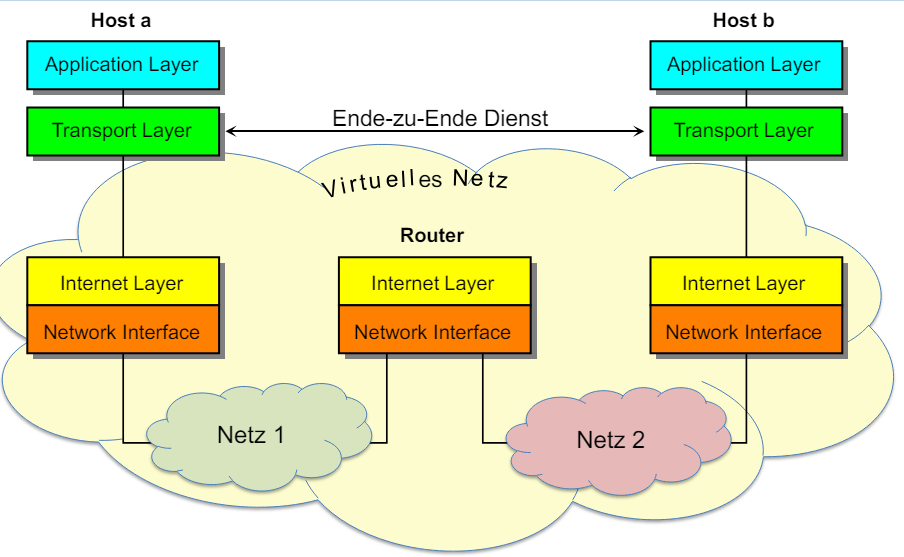
\includegraphics[width=0.75\linewidth]{images/images/transportlayer.png}

\begin{definition}{Transportlayer}\\
    Der Transport Layer bildet auch die Schnittstelle zwischen dem Betriebssystem (Kernel Space) und den Anwendungen (User Space)\\
    Der Zugriff auf die Funktionen des Transport Layers erfolgt via einer klar definierten Schnittstelle (Sockets)
\end{definition}

\begin{definition}{Kapselung}
    \begin{itemize}
        \item Die Applikationsdaten werden von den Protokollen des Transport Layers in ein IP-Paket gekapselt
        \item Das "Protocol" Feld unterscheidet UDP und TCP Daten
    \end{itemize}
    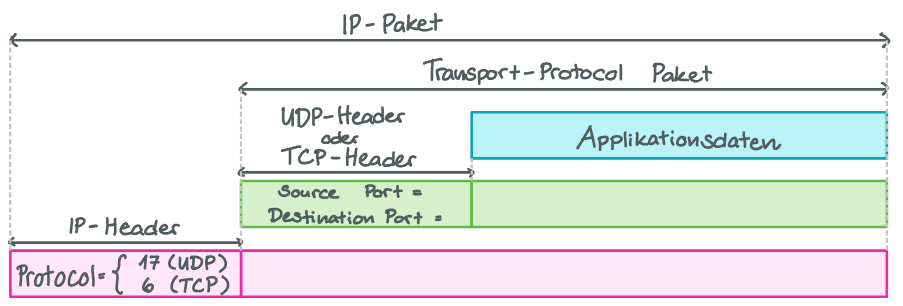
\includegraphics[width=1\linewidth]{images/images/tcp_udp_header.png}
\end{definition}

\begin{concept}{Adressierung der Applikation durch Port Nummern}\\
    Der Client adressiert mit der Destination Port Nummer die gewünschten Server-Applikation
    \begin{itemize}
        \item sonst weiss das TCP/UDP-Modul im Empfänger nicht, welche Applikation gemeint ist
        \item für die Source Port Nummer verwendet der Client (meist) eine zufällige Port Nummer im Bereich >1'023 (wird vom Betriebssystem vergeben)
    \end{itemize}
\end{concept}
    
\columnbreak

\subsection{UDP - User Datagram Protocol}

\begin{definition}{UDP}
    dient dem Multi- und Demultiplexen der Datagramme zu den Applikationen.
    \begin{itemize}
        \item Verbindungslos
        \item Unzuverlässig
    \end{itemize}
\end{definition}

\begin{concept}{UDP-Header}
    \begin{itemize}
        \item \textcolor{green}{Source Port} Sendende Applikation
        \item \textcolor{green}{Destination Port} Applikation des Empfängers
        \item \textcolor{blue}{Message Length} Länge des Datagramms
        \item \textcolor{purple}{Checksum} Prüfsumme über einen Pseudo-Header, UDP-Header und Daten
        \begin{itemize}
            \item kann Null sein
            \item Pseudo-Header: IP Source- und Destination Address, Protocol Feld, Länge des Datagramms
            \begin{itemize}
                \item so können fehlgeleitete Datagramme erkannt werden
                \item z.B. aufgrund eines Bit-Flip
            \end{itemize}
        \end{itemize}
    \end{itemize}
        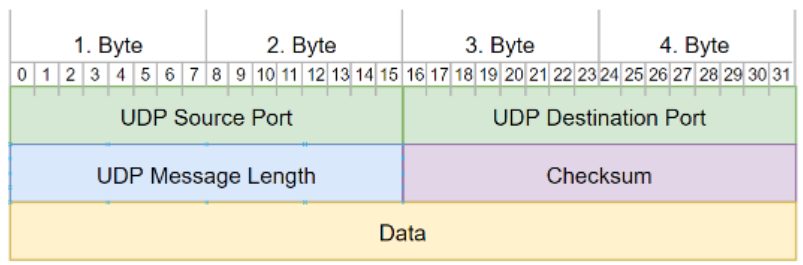
\includegraphics[width=1\linewidth]{images/images/udp.png}
\end{concept}

\begin{concept}{Adressierung und Multiplexing}\\
        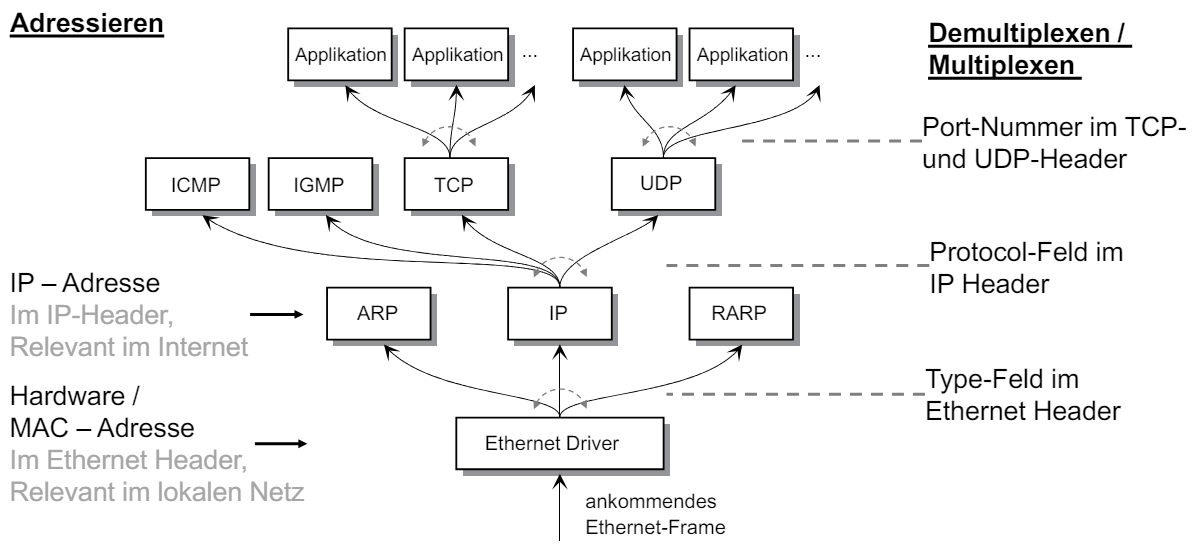
\includegraphics[width=1\linewidth]{images/images/adress_multiplex.png}
\end{concept}

\begin{formula}{Port-Nummern}
    \begin{itemize}
        \item \textcolor{green}{System Ports (Well-Known)} Feste Port-Nummern, für bekannte Appl. reserviert
        \item \textcolor{blue}{User Ports (Registered)} Reservierter Bereich für herstellerspezifische Appl.
        \item \textcolor{yellow}{Dynamic / Private Ports} Frei verfügbare Ports
    \end{itemize}
        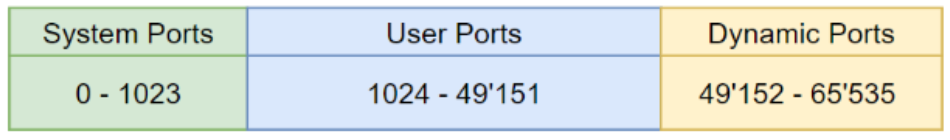
\includegraphics[width=1\linewidth]{images/images/portnummern.png}
\end{formula}

\subsection{TCP - Transmission Control Protocol}

\begin{definition}{TCP} Eigenschaften
    \begin{itemize}
        \item Verbindungsorientierte Übertragung: Zuerst wird eine Verbindung zwischen Client- und Serveranwendung aufgebaut
        \item Zuverlässiger Verbindungsaufbau: Bevor eine TCP-Verbindung steht, muss dies von beiden Endpunkten aktiv bestätigt werden
        \item Hohe Zuverlässigkeit: Die Daten kommen ohne Datenverlust und in der richtigen Reihenfolge auf der anderen Seite an
        \item Vollduplexübertragung: Gleichzeitige, voneinander unabhängige, Übertragung in beiden Richtungen möglich
        \item Stream-Schnittstelle: Die Anwendung sendet/empfängt eine unstrukturierte Byte-Folge
        \item Graceful Termination (Verbindungsabbau): TCP gewährt die Zustellung aller Daten auch beim Verbindungsabbau
        \item Punkt-zu-Punkt Kommunikation: Zwei Applikationen tauschen Daten aus. Konzepte wie Multicast oder Broadcast existieren nicht.
    \end{itemize}
\end{definition}

\begin{concept}{TCP-Header Format}
    \begin{itemize}
        \item \textcolor{yellow}{Sequence-Nr.} Nummer zur Ordnung der Segmente
        \item \textcolor{yellow}{Acknowledgement-Nr.} n + 1 → Daten bis und mit n korrekt und vollständig angekommen
        \item \textcolor{purple}{Data Offset} Gibt an wo Daten beginnen / enden
        \item \textcolor{purple}{ECN-Flags} Explicit Congestion Notification
        \begin{itemize}
            \item Bit 8: CWR (Congestion Window Reduced)
            \item Bit 9: ECE (ECN-Echo)
        \end{itemize}
        \item \textcolor{purple}{Control Bits} Verbindungsauf- und -abbau (Bits 10-15)
        URG: Urgent Pointer
        ACK: Acknowledgement Number
        PSH: Push (sofort ohne buffern weiterleiten)
        RST: Reset (Verbindung zurücksetzen oder geschlossenen Port signalisieren)
        SYN: Synchronize (Verbindung aufbauen)
        FIN: Verbindung abbauen
        \item \textcolor{blue}{Window} Verfügbare Puffergrösse (so viele Bytes dürfen noch gesendet werden)
        \item \textcolor{purple}{Urgent Pointer} URG = 1 → Position der wichtigen Daten
        \item \textcolor{purple}{Options} Häufigste Verwendung: MSS (Maximum Segment Size) die empfangen werden kann
    \end{itemize}
    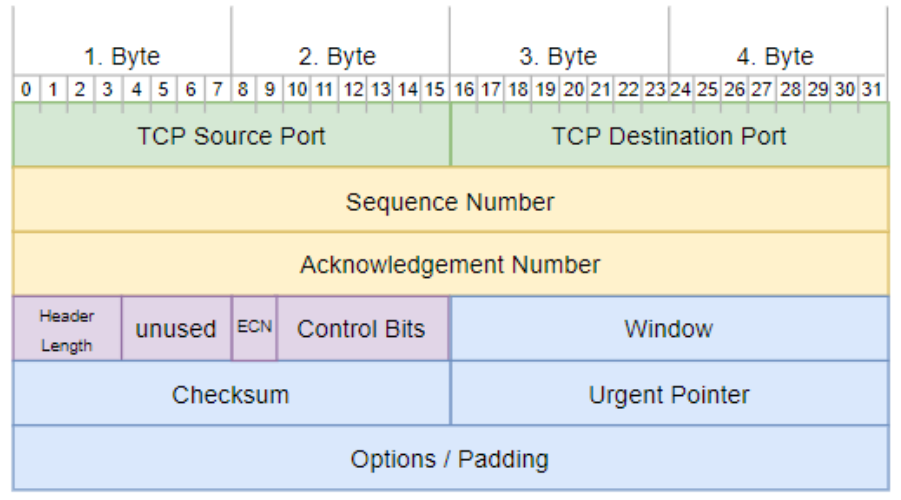
\includegraphics[width=1\linewidth]{images/images/tcpheader.png}
\end{concept}

\subsubsection{TCP Verkehrssteuerung}

\begin{concept}{Verbindungsorientierte Kommunikation}\\
    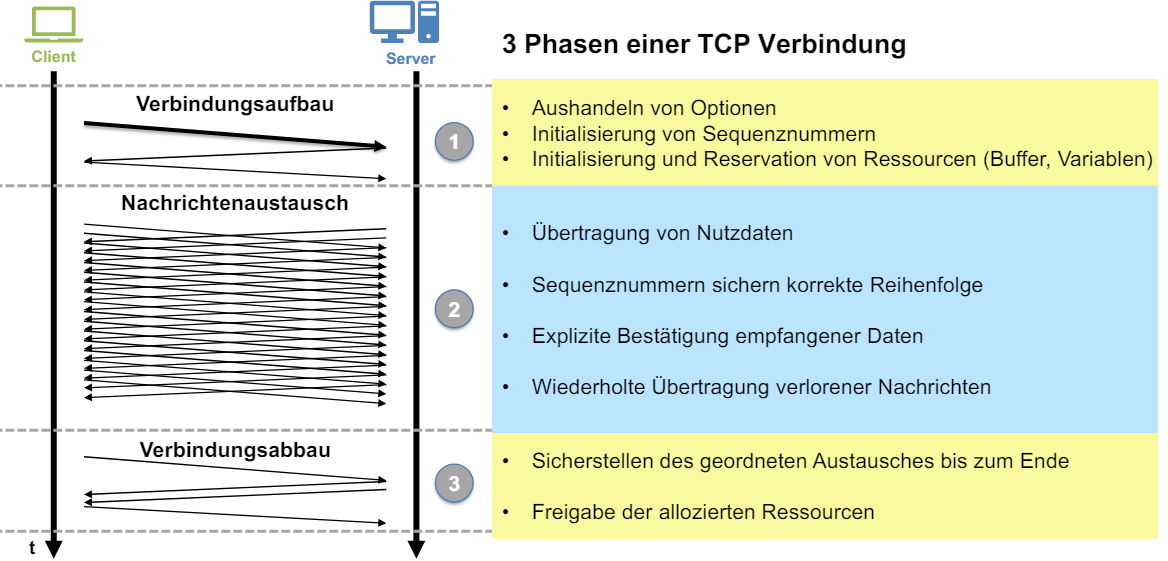
\includegraphics[width=1\linewidth]{images/images/verbindungsorientierte_kommunikation.png}
\end{concept}

\begin{concept}{Nachrichtenaustausch}\\
    Unabhängig für jede Richtung:
    \begin{itemize}
        \item Sequence Numbers (Senderichtung)
        \begin{itemize}
            \item Sicherstellen der richtigen Reihenfolge der Daten
            \item Erkennen verloren gegangener Daten
        \end{itemize}
        \item Acknowledge Numbers (Empfangsrichtung)
        \begin{itemize}
            \item Bestätigung korrekt empfangener Daten
            \item Erkennen verloren gegangener Daten
        \end{itemize}
        \item Flags steuern Verbindungsauf- und -abbau, signalisieren Gültigkeit von Informationen im Header und besondere Situationen.
        \begin{itemize}
            \item SYN/FIN: Verbindungsauf- und -abbau
            \item ACK: Acknowledge Number ist gültig
            \item PSH: Daten sollen schnellstmöglich weitergegeben werden
        \end{itemize}
    \end{itemize}
\end{concept}

\begin{definition}{Zustände}
    \begin{itemize}
        \item \textcolor{Goldenrod}{LISTEN} Auf Anforderung warten
        \item \textcolor{Goldenrod}{SYN-SENT} Anforderung geschickt
        \item \textcolor{Goldenrod}{SYN-RECEIVED} Anforderung erhalten
        \item \textcolor{green}{ESTABLISHED} Verbindung besteht
        \item \textcolor{Goldenrod}{FIN-WAIT-1} Abbauanforderung geschickt
        \item \textcolor{Goldenrod}{FIN-WAIT-2} Abbauanforderung bestätigt
        \item \textcolor{Goldenrod}{CLOSE-WAIT} Auf Lokale Verbindung warten
        \item \textcolor{Goldenrod}{LAST-ACK} Verbindungsabbau bestätigt
        \item \textcolor{Goldenrod}{TIME-WAIT} Letzte Bestätigung gesendet
    \end{itemize}
\end{definition}

\begin{concept}{Zustandsdiagramm}\\
    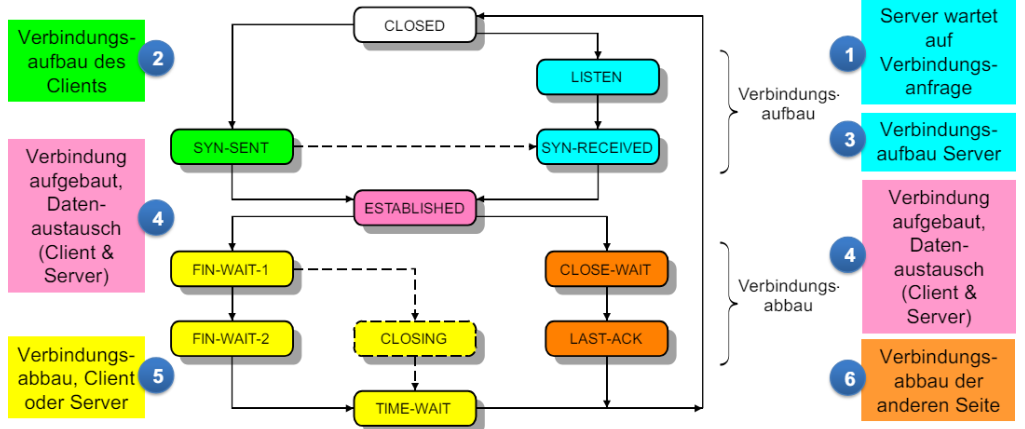
\includegraphics[width=1\linewidth]{images/images/zustandsdiagramm_tcp.png}
\end{concept}

\begin{KR}{Verbindungsaufbau}
    \begin{center}
        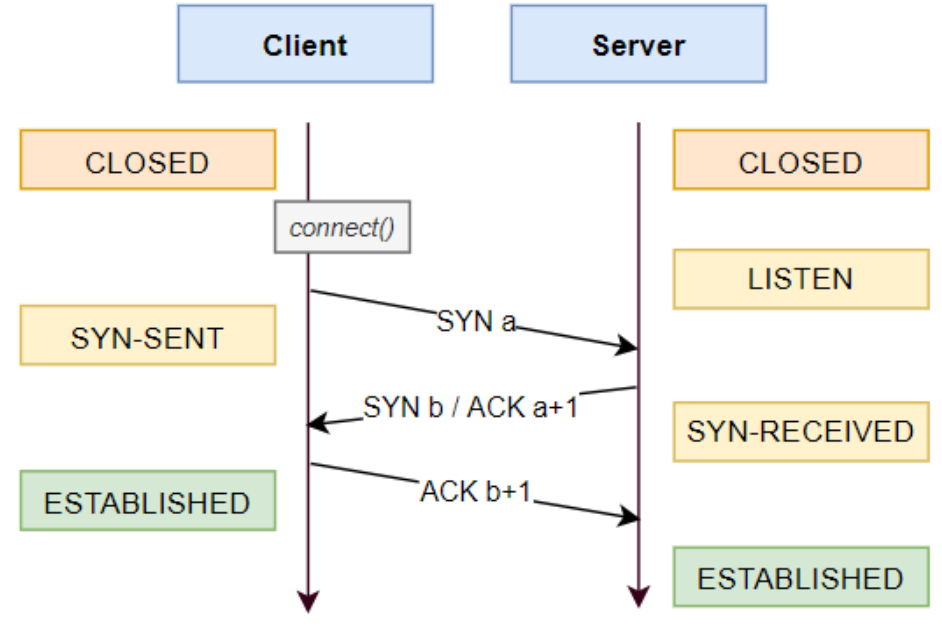
\includegraphics[width=0.7\linewidth]{images/images/verbindungsaufbau.png}
    \end{center}
\end{KR}

\begin{KR}{Datenaustausch}
    \begin{itemize}
        \item Nach dem Verbindungsaufbau können Daten geschickt werden
        \item Wenn der Server oder Client Daten schickt muss von dem anderen die Acknowledgement Nummer
        mit den Anzahl Bits der geschickten Daten aktualisieren
    \end{itemize}
\end{KR}

\begin{KR}{Verbindungsabbau}
    \begin{center}
        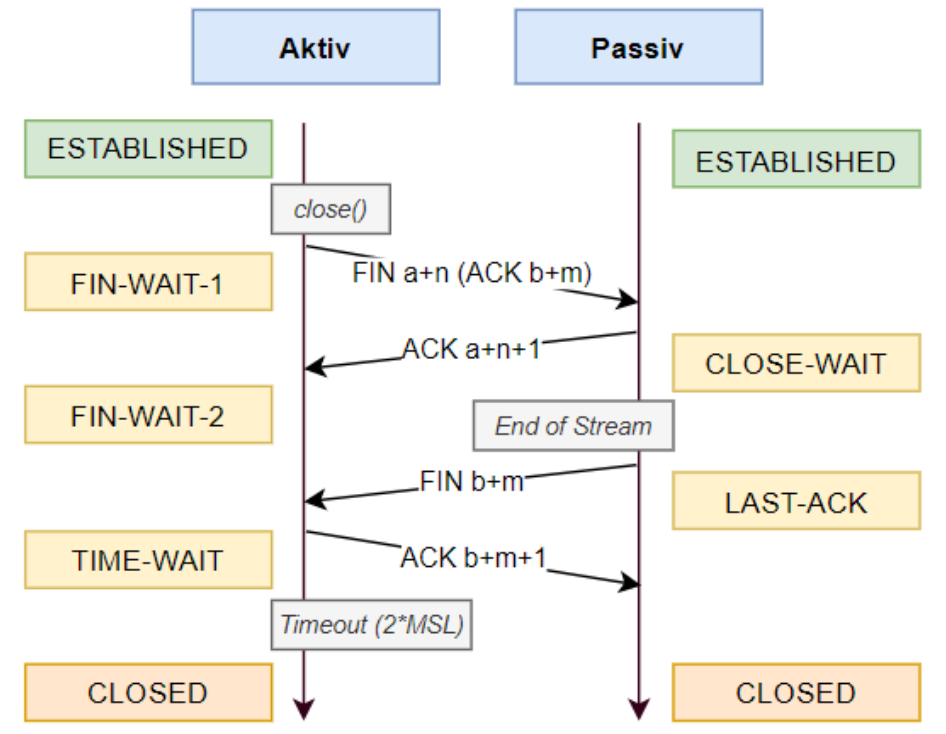
\includegraphics[width=0.7\linewidth]{images/images/Verbindungsabbau.png}
    \end{center}
\end{KR}

\begin{example2}{Datenaustausch}\\
    Geben Sie die Seq- und Ack-Nummern der Meldung M (1000 Bytes von Client zum Server) an und zeichnen Sie die entsprechenden Positionen ein. Beachten Sie, dass 1000 Bytes vom Server noch nicht vom Client empfangen wurden.\\
    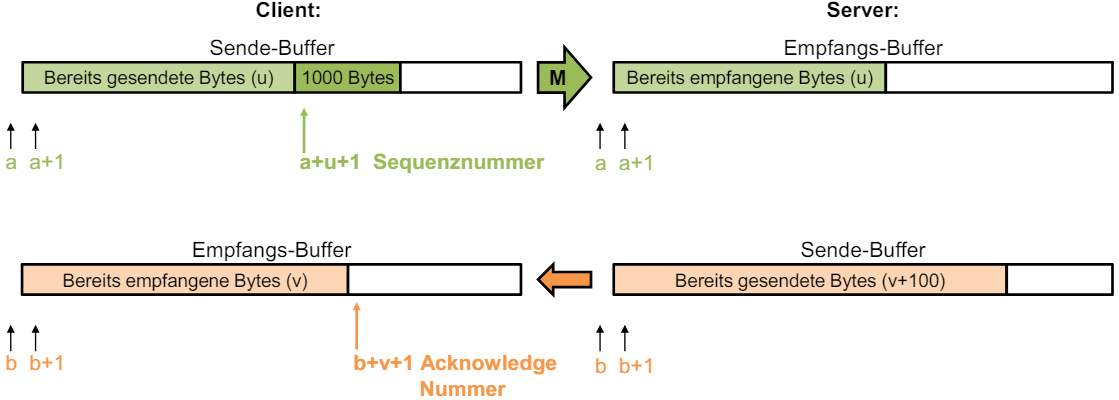
\includegraphics[width=1\linewidth]{images/images/datenaustausch_tcp_example.png}
\end{example2}

\subsubsection*{Vollständiges Beispiel}

\begin{example}
    Verbindungsaufbau:
    \begin{itemize}
        \item Server „horcht“ (LISTEN) auf einer bestimmten Port Nummer (z.B. 80 für einen HTTP Server)
        \item Client sendet Segment mit SYN=1 und zufälliger initialer Sequenznummer a (z. Bsp. 15'000) (ACK=0, weil Acknowledgement Nummer ungültig)
        \item Server bestätigt Sequenznummer mit Acknowledement Nummer a+1 (15'001) und ACK=1 und wählt zufällige initiale Sequenznummer b (z. Bsp. 42'300) und setzt SYN=1
        \item Client bestätigt b mit Acknowledement Nummer b+1 (42'301)
        \begin{itemize}
            \item Erstes Byte vom Client zum Server hat Sequenznummer a+1
            \item Erstes Byte vom Server zum Client hat Sequenznummer b+1
        \end{itemize}
    \end{itemize}
        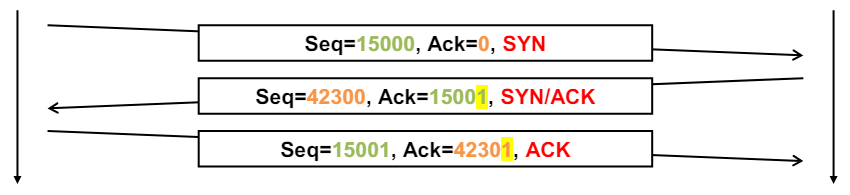
\includegraphics[width=1\linewidth]{images/images/example_verbindungsaufbau_tcp.png}
\end{example}

\begin{example}
    Während des Datenaustausches werden TCP-Nachrichten bi-direktional ausgetauscht
    \begin{itemize}
        \item Sequenznummer: Position des ersten Bytes der Daten im gesamten TCP-Datenstrom
        \item Acknowledgement Nummer: Sequenznummer des nächsten erwarteten Bytes
        \item ACK Flag: immer gesetzt
    \end{itemize}
        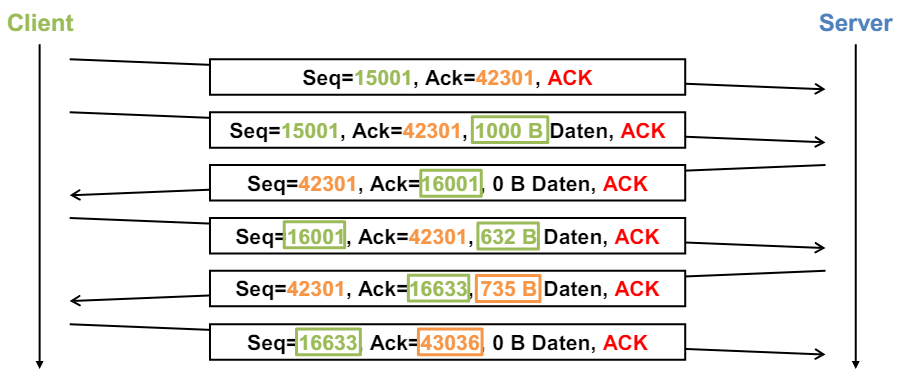
\includegraphics[width=1\linewidth]{images/images/tcp_datenaustausch_ex.png}
\end{example}

\begin{example}
    Beide Seiten können den Verbindungsabbau einleiten
    \begin{itemize}
        \item Ist eine Richtung geschlossen (FIN, ACK), so können in die andere Richtung immer noch Daten gesendet werden; dieser Verbindungszustand wird als Half-Closed bezeichnet.
        \begin{itemize}
            \item In Richtung der "geschlossenen" Verbindung wird nicht mehr kommuniziert (Acknowledge number mismatch)
        \end{itemize}
        \item Falls die zweite Seite die Verbindung auch schliesst, können die 3. und die 4. Nachricht zusammengefasst werden → FIN/ACK
    \end{itemize}
        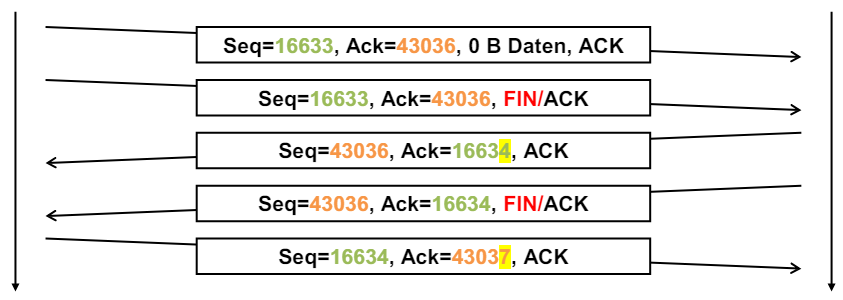
\includegraphics[width=1\linewidth]{images/images/tcp_verbindungsabbau_ex.png}
\end{example}





\subsection{TCP Adaptive Elemente}

\begin{formula}{Herausforderungen} zur Zuverlässigkeit zwischen Ethernet (Schicht 2) und TCP (Schicht 4):\\
    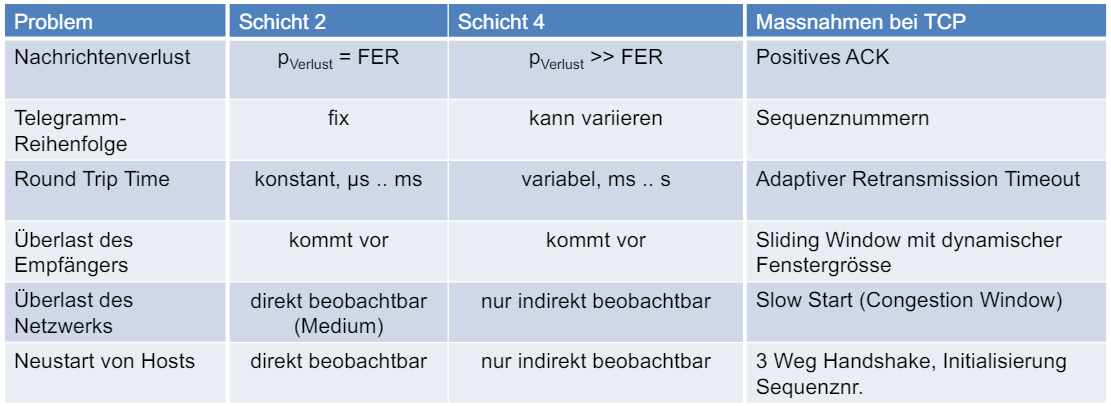
\includegraphics[width=1\linewidth]{images/vergleich_layer_2_4.png}
\end{formula}

\begin{definition}{Umgang mit dynamischen Situationen}
    \begin{itemize}
        \item Erkennung von verlorenen Telegrammen (Round Trip Time)
        \item Überlast des Empfängers (Fluss-Steuerung, Flow Control)
        \item Überlast des Netzes (Überlast-Steuerung, Congestion Control)
    \end{itemize}
\end{definition}

\subsubsection*{RTO - Round Trip Time Out}

\begin{formula}{Round Trip Time}
    dynamische Anpassung der Wartezeit bis
    zum senden des nächsten Pakets (Überlastung des
    Netztes). TCP misst bei jeder aktiven Verbindung
    die RTT und passt den RTO an.
    \vspace{1mm}
    \begin{itemize}
        \item Gewichteter Mittelwert \textcolor{blue}{SRTT (Smoothed Round-Trip Time)}
    \end{itemize}
    $$\alpha = 0.125: \textcolor{blue}{SRTT_n} = (1 - \alpha) \cdot \textcolor{blue}{SRTT_{n-1}} + \alpha \cdot \textcolor{green}{RTT_n}$$
    \begin{itemize}
        \item Streuung \textcolor{Goldenrod}{RTTVAR} des \textcolor{blue}{SRTT} der Abweichungen
    \end{itemize}
    $$\beta = 0.25: \textcolor{Goldenrod}{RTTVAR_n} = (1 - \beta) \cdot \textcolor{Goldenrod}{RTTVAR_{n-1}} + \beta \cdot \textcolor{blue}{SRTT_n} - \textcolor{green}{RTT_n}|$$
    \begin{itemize}
        \item Retransmission Time-Out RTO
    \end{itemize}
    $$RTO_n = \textcolor{blue}{SRTT_n} + 4 \cdot \textcolor{Goldenrod}{RTTVAR_n}$$
\end{formula}

\subsubsection*{Fluss-Steuerung und Congestion Control}

\begin{concept}{Fluss-Steuerung}\\
        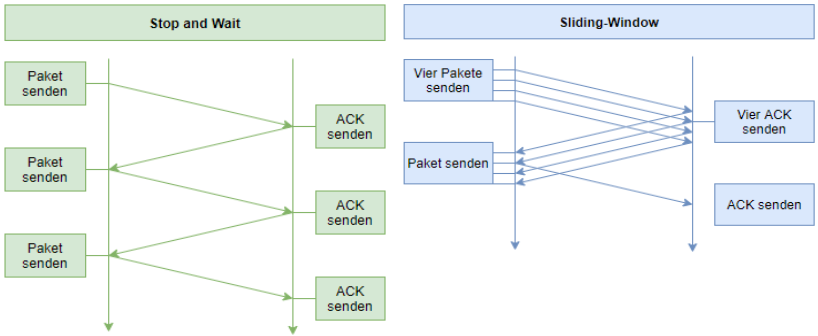
\includegraphics[width=1\linewidth]{images/images/fluss-steuerung.png}
\end{concept}





\begin{KR}{Sliding-Window TCP}
    \begin{itemize}
        \item Beide Richtungen arbeiten unabhängig voneinander
        \item Fenstergrösse wird in Anzahl Bytes angegeben
        \item Verbindungsaufbau: Initiale Fenstergrösse wird der anderen Seite mitgeteilt (Typische Werte: 16 / 32 / 64 KB)
        \item Pufferplatz im Empfänger wird alloziert
        \item Mit jedem ACK wird der verfügbare Pufferplatz (in Bytes) mitgeteilt und damit die Fenstergrösse dynamisch angepasst
        \item Fenstergrösse von 0 Bytes $\rightarrow$ keine Daten mehr senden
        \item Ist im Empfangsbuffer wieder Pufferplatz vorhanden, wird erneut eine Bestätigung mit diesem Pufferplatz an die andere Seite gesendet (= aktuelle Fenstergrösse)
    \end{itemize}
\end{KR}

\begin{formula}{Bandwidth Delay Product (TCP-Puffergrössen)}\\
    Wie gross sollten die Sende- und Empfangsbuffer gewählt werden, um eine TCP-Verbindung nicht auszubremsen?
    $$BDP (bits) = RTT (sec) \cdot Bandbreite (bps)$$
    RTT = Round-Trip-Time\\
    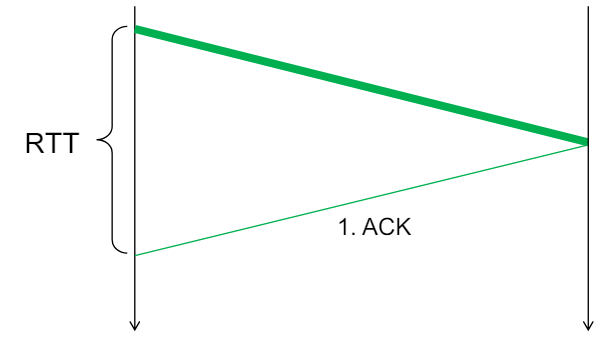
\includegraphics[width=0.3\linewidth]{images/images/bdp_rtt.png}
\end{formula}

\begin{example2}{Fluss-Steuerung bei TCP}\\
        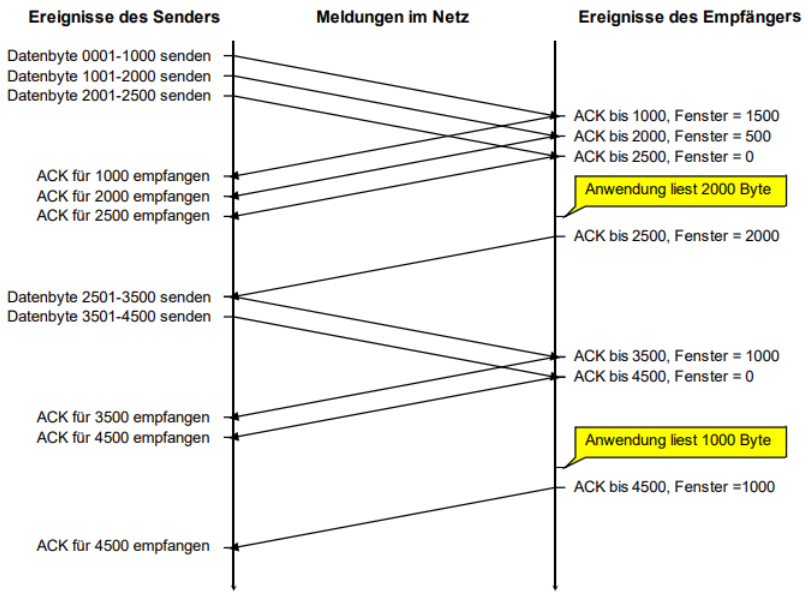
\includegraphics[width=1\linewidth]{images/images/flusssteuerung_tcp.png}\\
    Annahmen:
    \begin{itemize}
        \item 2'500 Byte Empfangspuffer
        \item 5'000 Bytes Daten
    \end{itemize}
    Ablauf:
    \begin{itemize}
        \item Fenstergrösse des Empfängers wird im WindowFeld des TCP-Headers übermittelt
        \item Wireshark gibt dieses als Advertized Window Size an
        \item Sender-Applikation benötigt nur einen Aufruf von send() für die gesamten 5'000 Bytes
    \end{itemize}
\end{example2}

\begin{concept}{Congestion Control - Slow Start}\\
    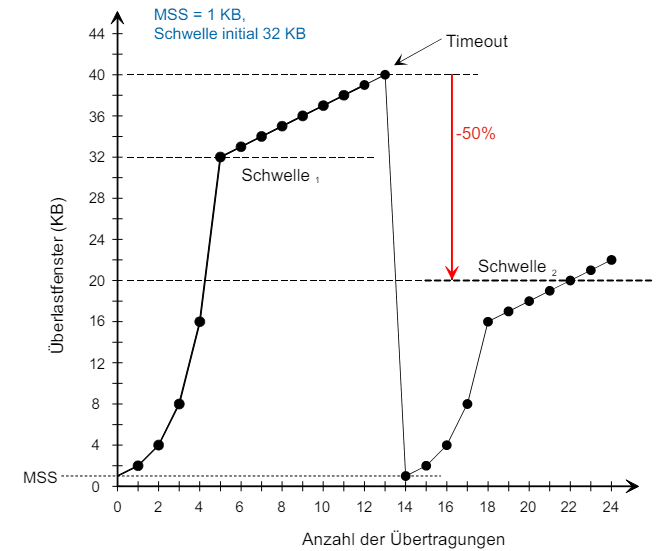
\includegraphics[width=0.75\linewidth]{images/images/congestion_control.png}\\
    Beim Slow Start wird heran getastet wie gross die einzelnen Frames sein können.\\
    \textbf{Wichtig:} Der Sender kombiniert das Congestion Window mit den Informationen zur Flow Control vom Empfänger und schickt unbestätigte Daten bis zum Erreichen von: min \{Congestion Window, Advertised Window\}
\end{concept}

